\documentclass{article}
\usepackage[margin=1in]{geometry}
\usepackage{amsmath,amsthm,amssymb}
\usepackage{bbm,enumerate,mathtools}
\usepackage{tikz,pgfplots}
\usepackage{chessboard}
\usepackage[hidelinks]{hyperref}
\usepackage{multicol} % Problem 35

\newenvironment{question}{\begin{trivlist}\item[\textbf{Question.}]}{\end{trivlist}}
\newenvironment{note}{\begin{trivlist}\item[\textbf{Note.}]}{\end{trivlist}}
\newenvironment{references}{\begin{trivlist}\item[\textbf{References.}]}{\end{trivlist}}
\newenvironment{related}{\begin{trivlist}\item[\textbf{Related.}]\end{trivlist}\begin{enumerate}}{\end{enumerate}}

\usepackage{pgfplots}

\begin{document}
\rating{2}{2}
Let $h$ be the maximum number of penny-to-penny connections on the vertices of
a hexagonal lattice, and let $t(n)$ be the analogous sequence on the vertices of
a triangular lattice.
\begin{figure}[!h]
  \centering
  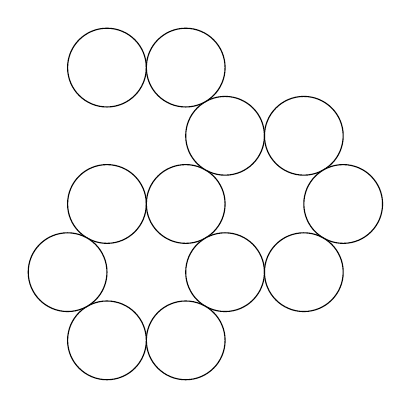
\begin{tikzpicture}
    \draw[fill=white] (-0.5,{sqrt(3)/2}) circle (0.5cm);
    \draw[fill=white] (0.5,{sqrt(3)/2}) circle (0.5cm);
    \draw[fill=white] (1,0) circle (0.5cm);
    \draw[fill=white] (0.5,{-sqrt(3)/2}) circle (0.5cm);
    \draw[fill=white] (-0.5,{-sqrt(3)/2}) circle (0.5cm);
    \draw[fill=white] (-1,0) circle (0.5cm);

    \draw[fill=white] (1,{sqrt(3)}) circle (0.5cm);
    \draw[fill=white] (2,{sqrt(3)}) circle (0.5cm);
    \draw[fill=white] (2.5,{sqrt(3)/2}) circle (0.5cm);
    \draw[fill=white] (2,0) circle (0.5cm);

    \draw[fill=white] (-0.5,{3*sqrt(3)/2}) circle (0.5cm);
    \draw[fill=white] (0.5,{3*sqrt(3)/2}) circle (0.5cm);
  \end{tikzpicture}\hspace{1cm}
  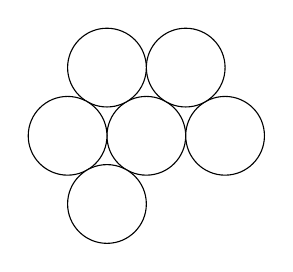
\begin{tikzpicture}
    \draw[fill=white] (0,0) circle (0.5cm);
    \draw[fill=white] (1,0) circle (0.5cm);
    \draw[fill=white] (0.5,{sqrt(3)/2}) circle (0.5cm);
    \draw[fill=white] (-0.5,{sqrt(3)/2}) circle (0.5cm);
    \draw[fill=white] (-1,0) circle (0.5cm);
    \draw[fill=white] (-0.5,{-sqrt(3)/2}) circle (0.5cm);
  \end{tikzpicture}
  \caption{
    An example for $h(12)=13$ and $t(6)=9$
  }
\end{figure}

\begin{question}
  What is a combinatorial proof that $h(2n) - t(n) = A216256(n)$.
\end{question}

\begin{note}
  A216256 is \[
    \underbrace{1}_1,
    \underbrace{2}_1,
    \underbrace{3, 3}_2,
    \underbrace{4, 4, 4}_3,
    \underbrace{5, 5, 5}_3,
    \underbrace{6, 6, 6, 6}_4,
    \underbrace{7, 7, 7, 7, 7}_5,
    \underbrace{8, 8, 8, 8, 8}_5,
    \underbrace{9, 9, 9, 9, 9, 9}_6, \hdots
  \]
\end{note}

\begin{related}
  \item \url{https://oeis.org/A216256}
  \item $t(n)$: \url{https://oeis.org/A047932}
  \item $h(n)$: \url{https://oeis.org/A263135}
\end{related}
\end{document}
